\section{Experiments}
\label{sec:experiment}

We present empirical evaluations for cold-start playlist recommendation on two real playlist datasets,
and compare the proposed multitask learning method with a number of well known baseline approaches.
%In this section, we describe experiments that empirically evaluate the proposed method and a number of 
%well known baseline approaches in the three cold-start settings. %described in Section~\ref{sec:problem}.


\subsection{Dataset}
%We make use of 
%We use
We evaluate on 
two publicly available playlist datasets: the 30Music~\cite{30music2015} and 
the AotM-2011~\cite{mcfee2012hypergraph} dataset.
The Million Song Dataset (MSD)~\cite{msd2011} serves as an underlying dataset where songs in all playlists 
are intersected; additionally, song and artist information in the MSD are used to compute song features.
%Additionally, song metadata (\eg song title, artist name, year of release) and precomputed audio features 
%in MSD are employed to compute song features.

 
%It also provides a few song features which will be described later in this section.
%Million Song Dataset (MSD) is a collection of one million songs, where each song is described by its metadata 
%(\eg song title, artist name, year of release) and a number of precomputed audio features from the Echo Nest\footnote{http://the.echonest.com}.
%It also provides acoustic features computed from a sample section of audio file of each song. % more description


%\begin{table}[hbt]
%\centering
%\caption{Music playlist dataset}
%\label{tab:stats_pldata}
%\resizebox{\linewidth}{!}{
%\setlength\tabcolsep{3pt}
%\begin{tabular}{lrcrrccc}
%\toprule
%Dataset   & Songs   & Playlists & Users   & Artists & Songs/Playlist & Playlists/User & Songs/Artist \\
%\midrule                                                                                             
%30Music   & 45,468  & 17,457    & 8,070   & 9,981   & 16.3           & 2.2            & 28.6 \\
%AotM-2011 & 114,428 & 84,710    & 14,182  & 15,698  & 10.1           & 6.0            & 53.8 \\
%\bottomrule
%\end{tabular}
%}
%\end{table}

%\begin{table*}[!t]
    \centering
    \begin{minipage}{.35\textwidth}
        \centering
        \caption{Dataset for \emph{cold songs}}
        \label{tab:stats0}
        \resizebox{.9\textwidth}{!}{
        \begin{tabular}{lrrcrr}
        \toprule
        \multirow{2}{*}{Dataset}  & \multicolumn{2}{c}{Songs} && \multicolumn{2}{c}{Playlists} \\ \cmidrule{2-3} \cmidrule{5-6}
                                  & Train & Test && Train & Test \\
        \midrule
        30Music   & 40,468  & 5,000  && 17,342  & 8,215 \\
        AotM-2011 & 104,428 & 10,000 && 84,646  & 19,504 \\
        \bottomrule
        \end{tabular}
        }
    \end{minipage}%
    \begin{minipage}{0.33\textwidth}
        \centering
        \caption{Dataset for \emph{cold playlists}}
        \label{tab:stats1}
        \resizebox{.9\textwidth}{!}{
        \begin{tabular}{lrrcrr}
        \toprule
        \multirow{2}{*}{Dataset}  & \multicolumn{2}{c}{Playlists} && \multicolumn{2}{c}{Users} \\ \cmidrule{2-3} \cmidrule{5-6}
                                  & Train & Test && Train & Test \\
        \midrule
        30Music   & 15,262 & 2,195 &&  8,070 & 1,644 \\
        AotM-2011 & 75,477 & 9,233 && 14,182 & 2,722 \\
        \bottomrule
        \end{tabular}
        }
    \end{minipage}%
    \begin{minipage}{.33\textwidth}
        \centering
        \caption{Dataset for \emph{cold users}}
        \label{tab:stats2}
        \resizebox{.9\textwidth}{!}{
        \begin{tabular}{lrrcrr}
        \toprule
        \multirow{2}{*}{Dataset}  & \multicolumn{2}{c}{Playlists} && \multicolumn{2}{c}{Users} \\ \cmidrule{2-3} \cmidrule{5-6}
                                  & Train & Test && Train & Test \\
        \midrule
        30Music   & 14,067 & 3,390 && 5,649 & 2,421 \\
        AotM-2011 & 76,450 & 8,260 && 9,928 & 4,254 \\
        \bottomrule
        \end{tabular}
        }
    \end{minipage}
\end{table*}


\noindent
{\bf 30Music Dataset} is a collection of listening events and user-generated
playlists retrieved from Last.fm.\footnote{https://www.last.fm}
We first intersect the playlists data with songs in the MSD, 
%leveraging the Last.fm dataset~\cite{lastfmdataset} which matched songs from Last.fm with those in the MSD, 
then filter out playlists with less than 5 songs.
This results in about 17K playlists over 45K songs from 8K users.

\noindent
{\bf AotM-2011 Dataset} is a collection of playlists shared by Art of the Mix\footnote{http://www.artofthemix.org} 
users during the period from 1998 to 2011. Songs in playlists have been matched to those in the MSD.
%We filter out playlists with less than 5 songs, which results in 
It contains 
roughly 84K playlists over 114K songs from 14K users
after filtering out playlists with less than 5 songs.

Table~\ref{tab:stats_pldata} summarises the two 
playlist datasets used in this work.
See Appendix for more details.


%\subsubsection{Features}
\subsection{Features}

% of songs used in the experiments include metadata, audio data, genre and artist information, as well as song and 
Song metadata, audio data, genre and artist information, as well as song popularity
(\ie the accumulated playcount of the song in the training set)
and artist popularity 
(\ie the accumulated playcount of all songs from the artist in the training set)
are encoded as features.
%
The metadata of songs (\eg duration, year of release) and pre-computed audio features (\eg loudness, mode, tempo) are from the MSD.
%provided by the MSD.
We use genre data from the Top-MAGD genre dataset~\cite{schindler2012facilitating}
and tagtraum genre annotations for the MSD~\cite{schreiber2015improving} via one-hot encoding.
%If the genre data of a song is not available, 
If the genre of a song is unknown, 
we apply mean imputation using genre counts of songs in the training set.
To encode artist information as features,
we create a sequence of artist identifiers for each playlist in the training set, and train
%we trained 
a word2vec\footnote{https://github.com/dav/word2vec} model that learns embeddings of artists.
% of artist identifiers in training playlists.
%
We assume no popularity information is available for newly released songs,
and therefore song popularity is not a feature in the \emph{cold songs} setting.
%thus song popularity is used as a feature only in the \emph{cold playlists} and \emph{cold users} settings.
%In the task of recommending new songs to extend existing playlists (setting (i)), where song popularity is not available,
%we use artist popularity (we use the number of occurrences of all songs from a artist in training playlists as a proxy of her popularity).
Finally, we add a constant feature (with value $1.0$) for each song to account for bias.


\begin{table}[!t]
\centering
\caption{Statistics of music playlist datasets}
\label{tab:stats_pldata}
\resizebox{.8\linewidth}{!}{
%\setlength\tabcolsep{3pt}
\begin{tabular}{lrr}
\toprule
               & 30Music & AotM-2011 \\
\midrule
Playlists      & 17,457  & 84,710    \\
Users          & 8,070   & 14,182    \\
Avg. Playlists per User & 2.2     & 6.0       \\
\midrule
Songs          & 45,468  & 114,428   \\
Avg. Songs per Playlist & 16.3    & 10.1      \\
\midrule
Artists        & 9,981   & 15,698    \\
Avg. Songs per Artist   & 28.6    & 53.8      \\
\bottomrule
\end{tabular}
}
\end{table}



\subsection{Experimental setup}

We split the two playlist datasets into training and test sets, %for each of the three cold-start settings,
evaluate the test set performance of the proposed method,
and compare it against
%and compare the test set performance of the proposed method with that of 
several baseline approaches
%and compare the proposed multitask learning method with several baseline approaches
in each of the three cold-start settings.

%We describe how playlists in the two datasets are split into training and test set for the three cold-start settings,
%and the features of songs used to learn the multitask objective, as well as baseline approaches and evaluation metrics.

\subsubsection{Dataset split}
%For the task of recommending songs to form new playlists for existing users (\ie the \emph{cold playlists} setting),
In the \emph{cold playlists} setting,
%To empirically evaluate the performance of our proposed recommendation approaches for existing users,
we hold a portion of the playlists from about 20\% of users in both datasets for testing, 
and all other playlists are used for training.
The test set is formed by sampling playlists where each song has been included in 
at least five playlists among the whole dataset.
We also make sure each song in the test set appears in the training set,
and all users in the test set have a few %a number of 
playlists in the training set.
%This results in about 2.1K playlists from 1.6K users for test in the 30Music dataset,
%and about 9.2K playlists from 2.7K users for test in the AotM-2011 dataset.
%This results in a test set with about 2.1K playlists from 1.6K users in 30Music dataset,
%and a test set with about 9.2K playlists from 2.7K users in AotM-2011 dataset.
%The statistics of this training/test split are shown in Table~\ref{tab:stats1}.
%Table~\ref{tab:stats1} summarises this split. %training and test split. % of the two playlist datasets. 
%
In the \emph{cold users} setting,
%To evaluate the task of recommending songs for new users to form playlists (\ie the \emph{cold users} setting),
%To evaluate the performance of music recommendation approaches for new users,
we sample 30\% of users and hold all of their playlists in both datasets.
Similarly, we require songs in the test set to appear in the training set,
and a user will thus not be used for testing %included in the test set 
if holding all of her playlists breaks this requirement.
%This results in about 3.4K playlists from 2.4K users for test in the 30Music dataset,
%and about 8.2K playlists from 4.2K users for test in the AotM-2011 dataset.
%This results in a test set with about 3.4K playlists from 2.4K users in 30Music dataset,
%and a test set with about 8.2K playlists from 4.2K users in AotM-2011 dataset.
%Table~\ref{tab:stats2} describes the statistics of this split. %training and test split.
%
%To empirically evaluate the performance of recommending new songs to extend existing playlists (\ie the \emph{cold songs} setting),
To evaluate 
in the \emph{cold songs} setting,
we hold 5K of the latest released songs in the 30Music dataset,
and 10K of the latest released songs in the AotM-2011 dataset where more songs are available.
%This results in about 8K playlists with songs in both the training and test set.
%In the AotM-2011 dataset where more songs are available, we hold 10K of the latest released songs.
%This leads to about 19K playlists with songs in both the training and test set.
We remove playlists where all songs have been held for testing. %are removed from both the training and test set.
%This results in about 8K playlists in the 30Music dataset and about 19K playlists in the AotM-2011 dataset.
%Table~\ref{tab:stats0} shows the statistics of this split. %training and test split.

See Appendix for the statistics of these dataset splits.
%See Appendix for the statistics of these training and test splits.
%Table~\ref{tab:stats1} summarises this split. %training and test split. % of the two playlist datasets. 


%\begin{figure*}[!t]
    \centering
    \begin{minipage}{.32\textwidth}
        \centering
        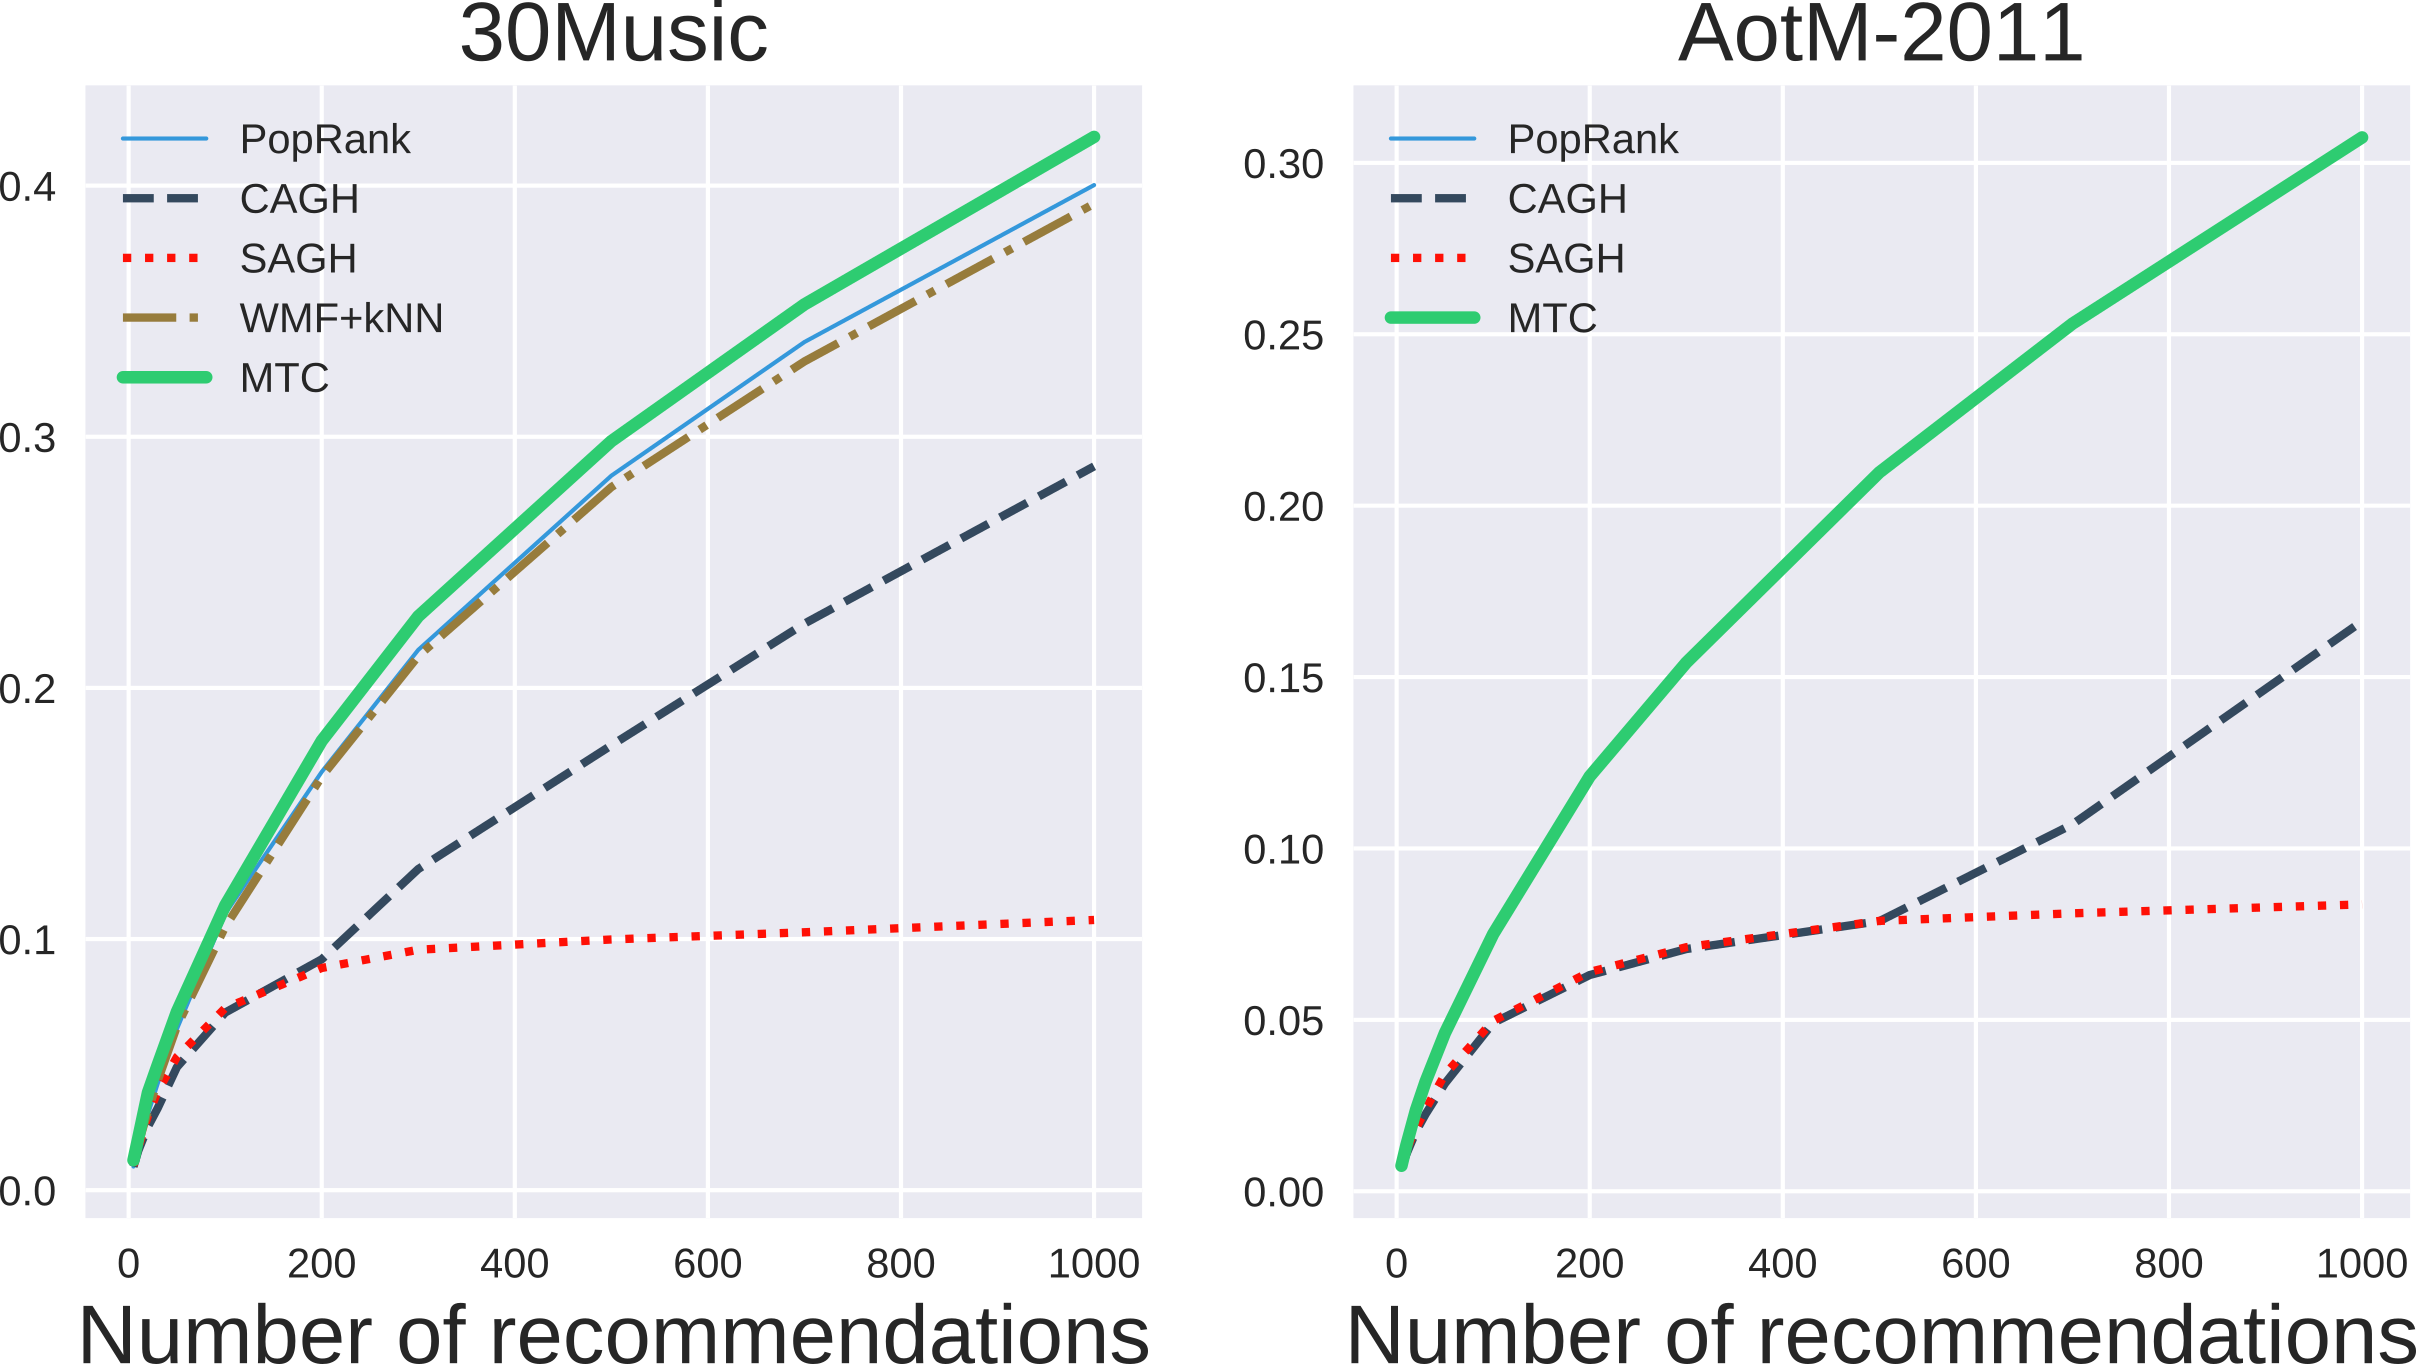
\includegraphics[width=.96\linewidth]{fig/hr4.png}
        \caption{Hit rates for {\it cold users}}
        \label{fig:hr4}
    \end{minipage}\hspace{11pt}%
    \begin{minipage}{0.32\textwidth}
        \centering
        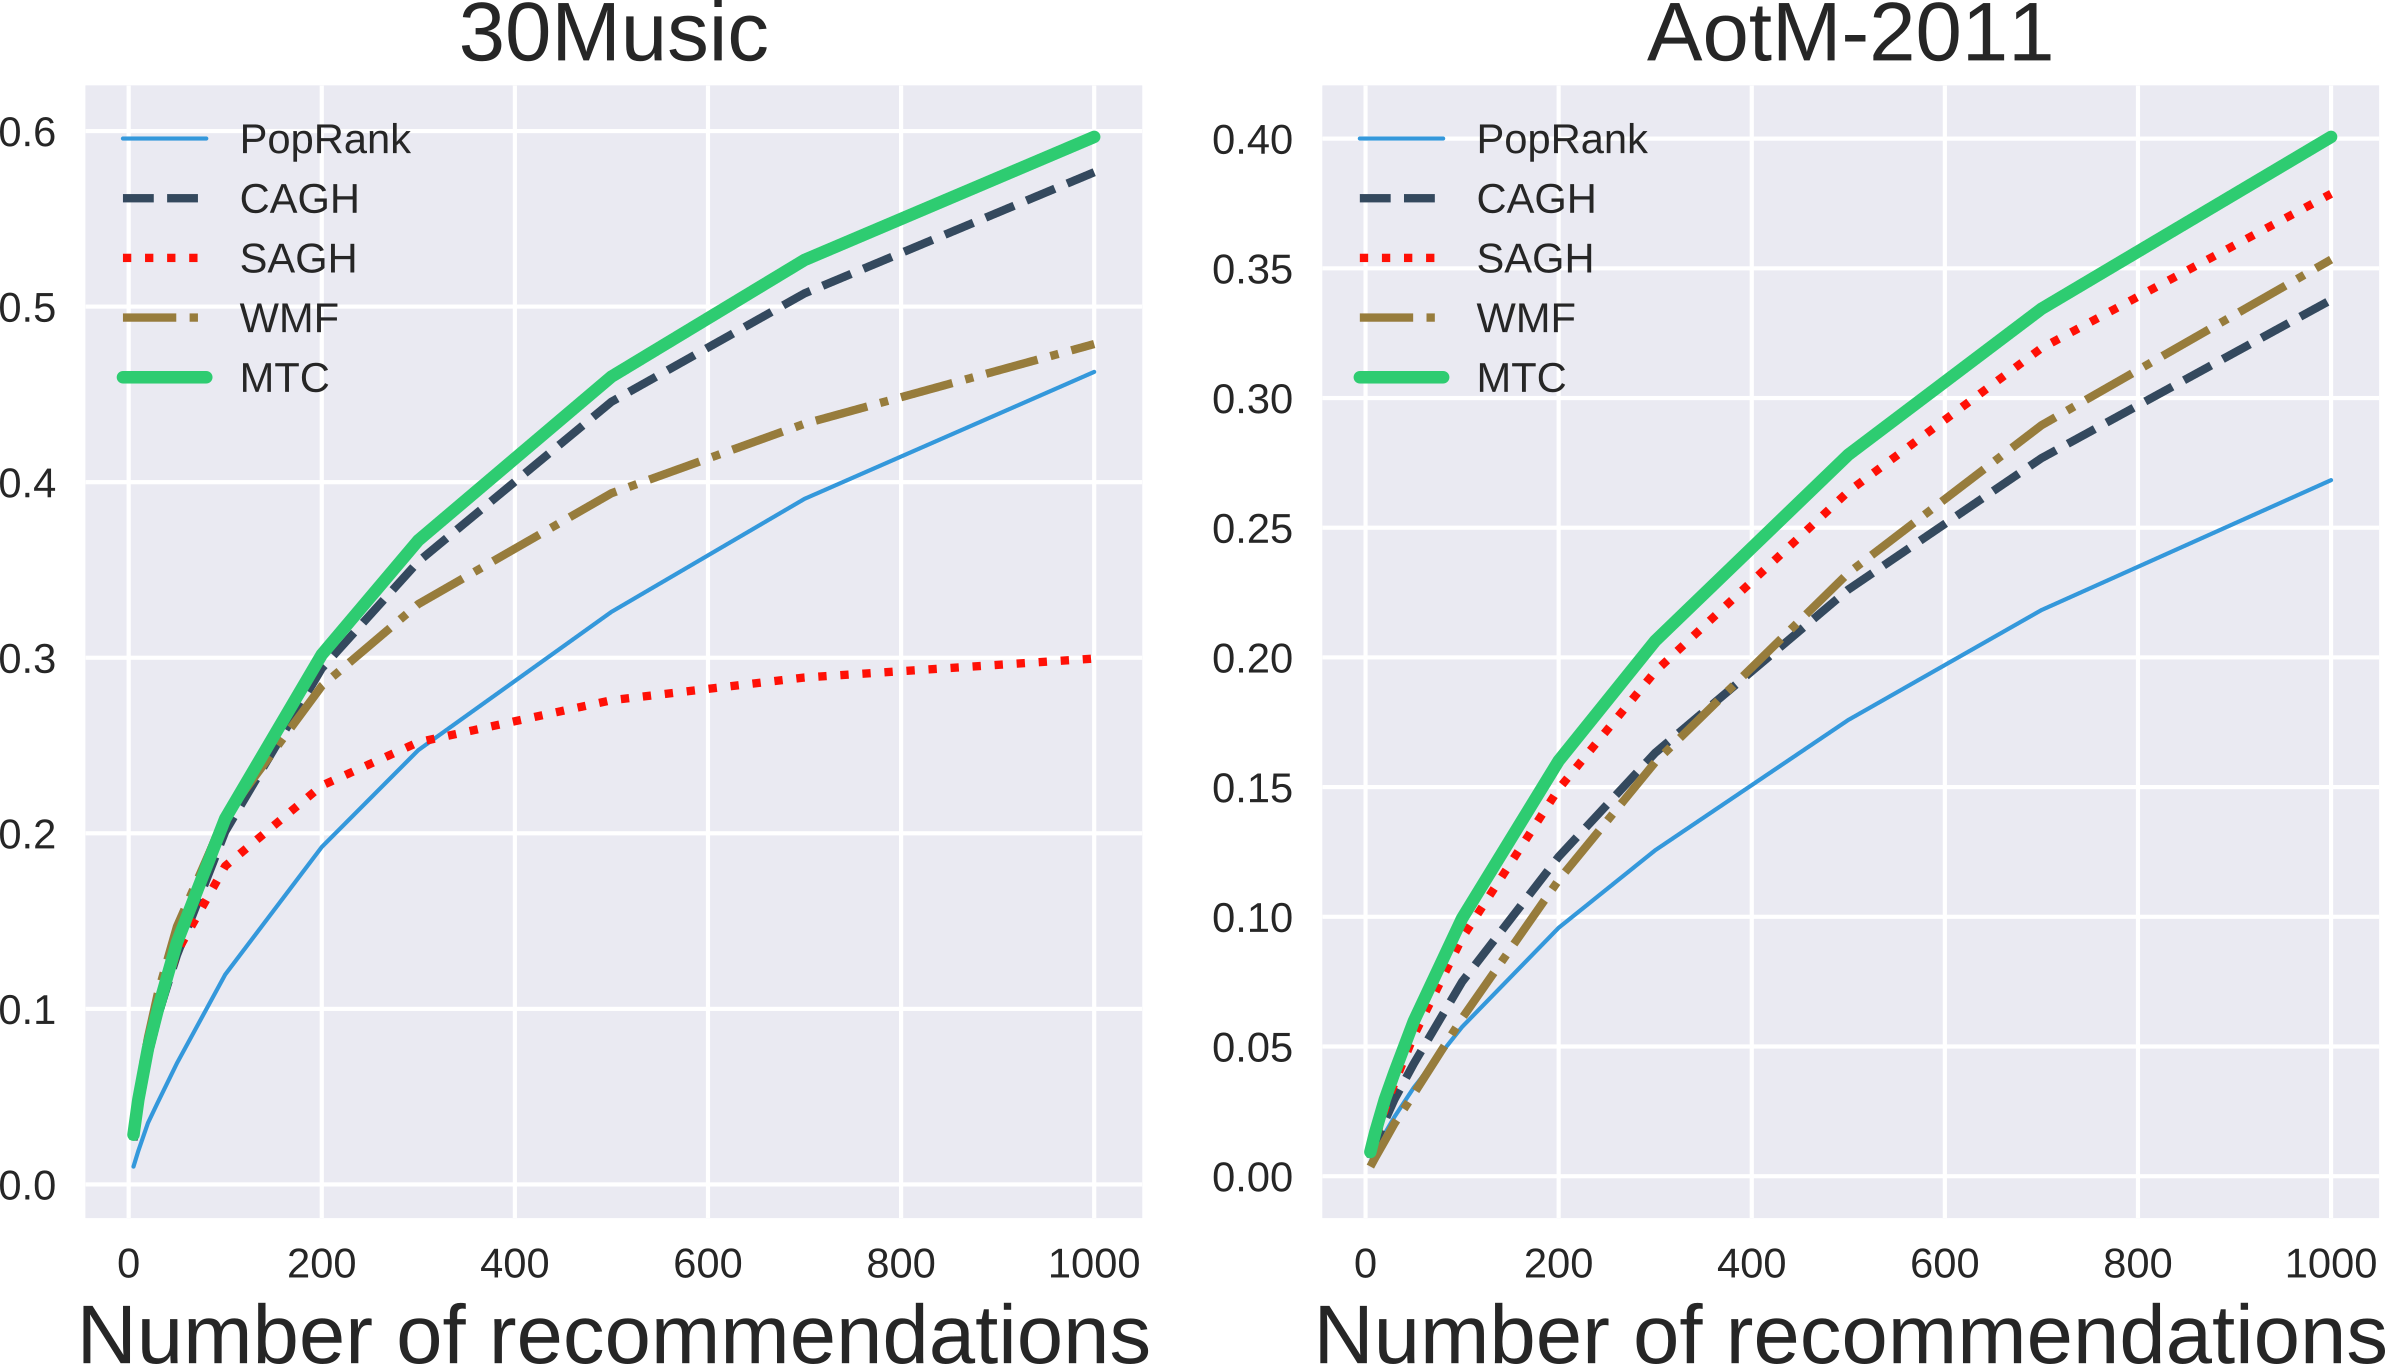
\includegraphics[width=.96\linewidth]{fig/hr3.png}
        \caption{Hit rates for {\it cold playlists}}
        \label{fig:hr3}
    \end{minipage}\hspace{8pt}%
    \begin{minipage}{0.32\textwidth}
        \centering
        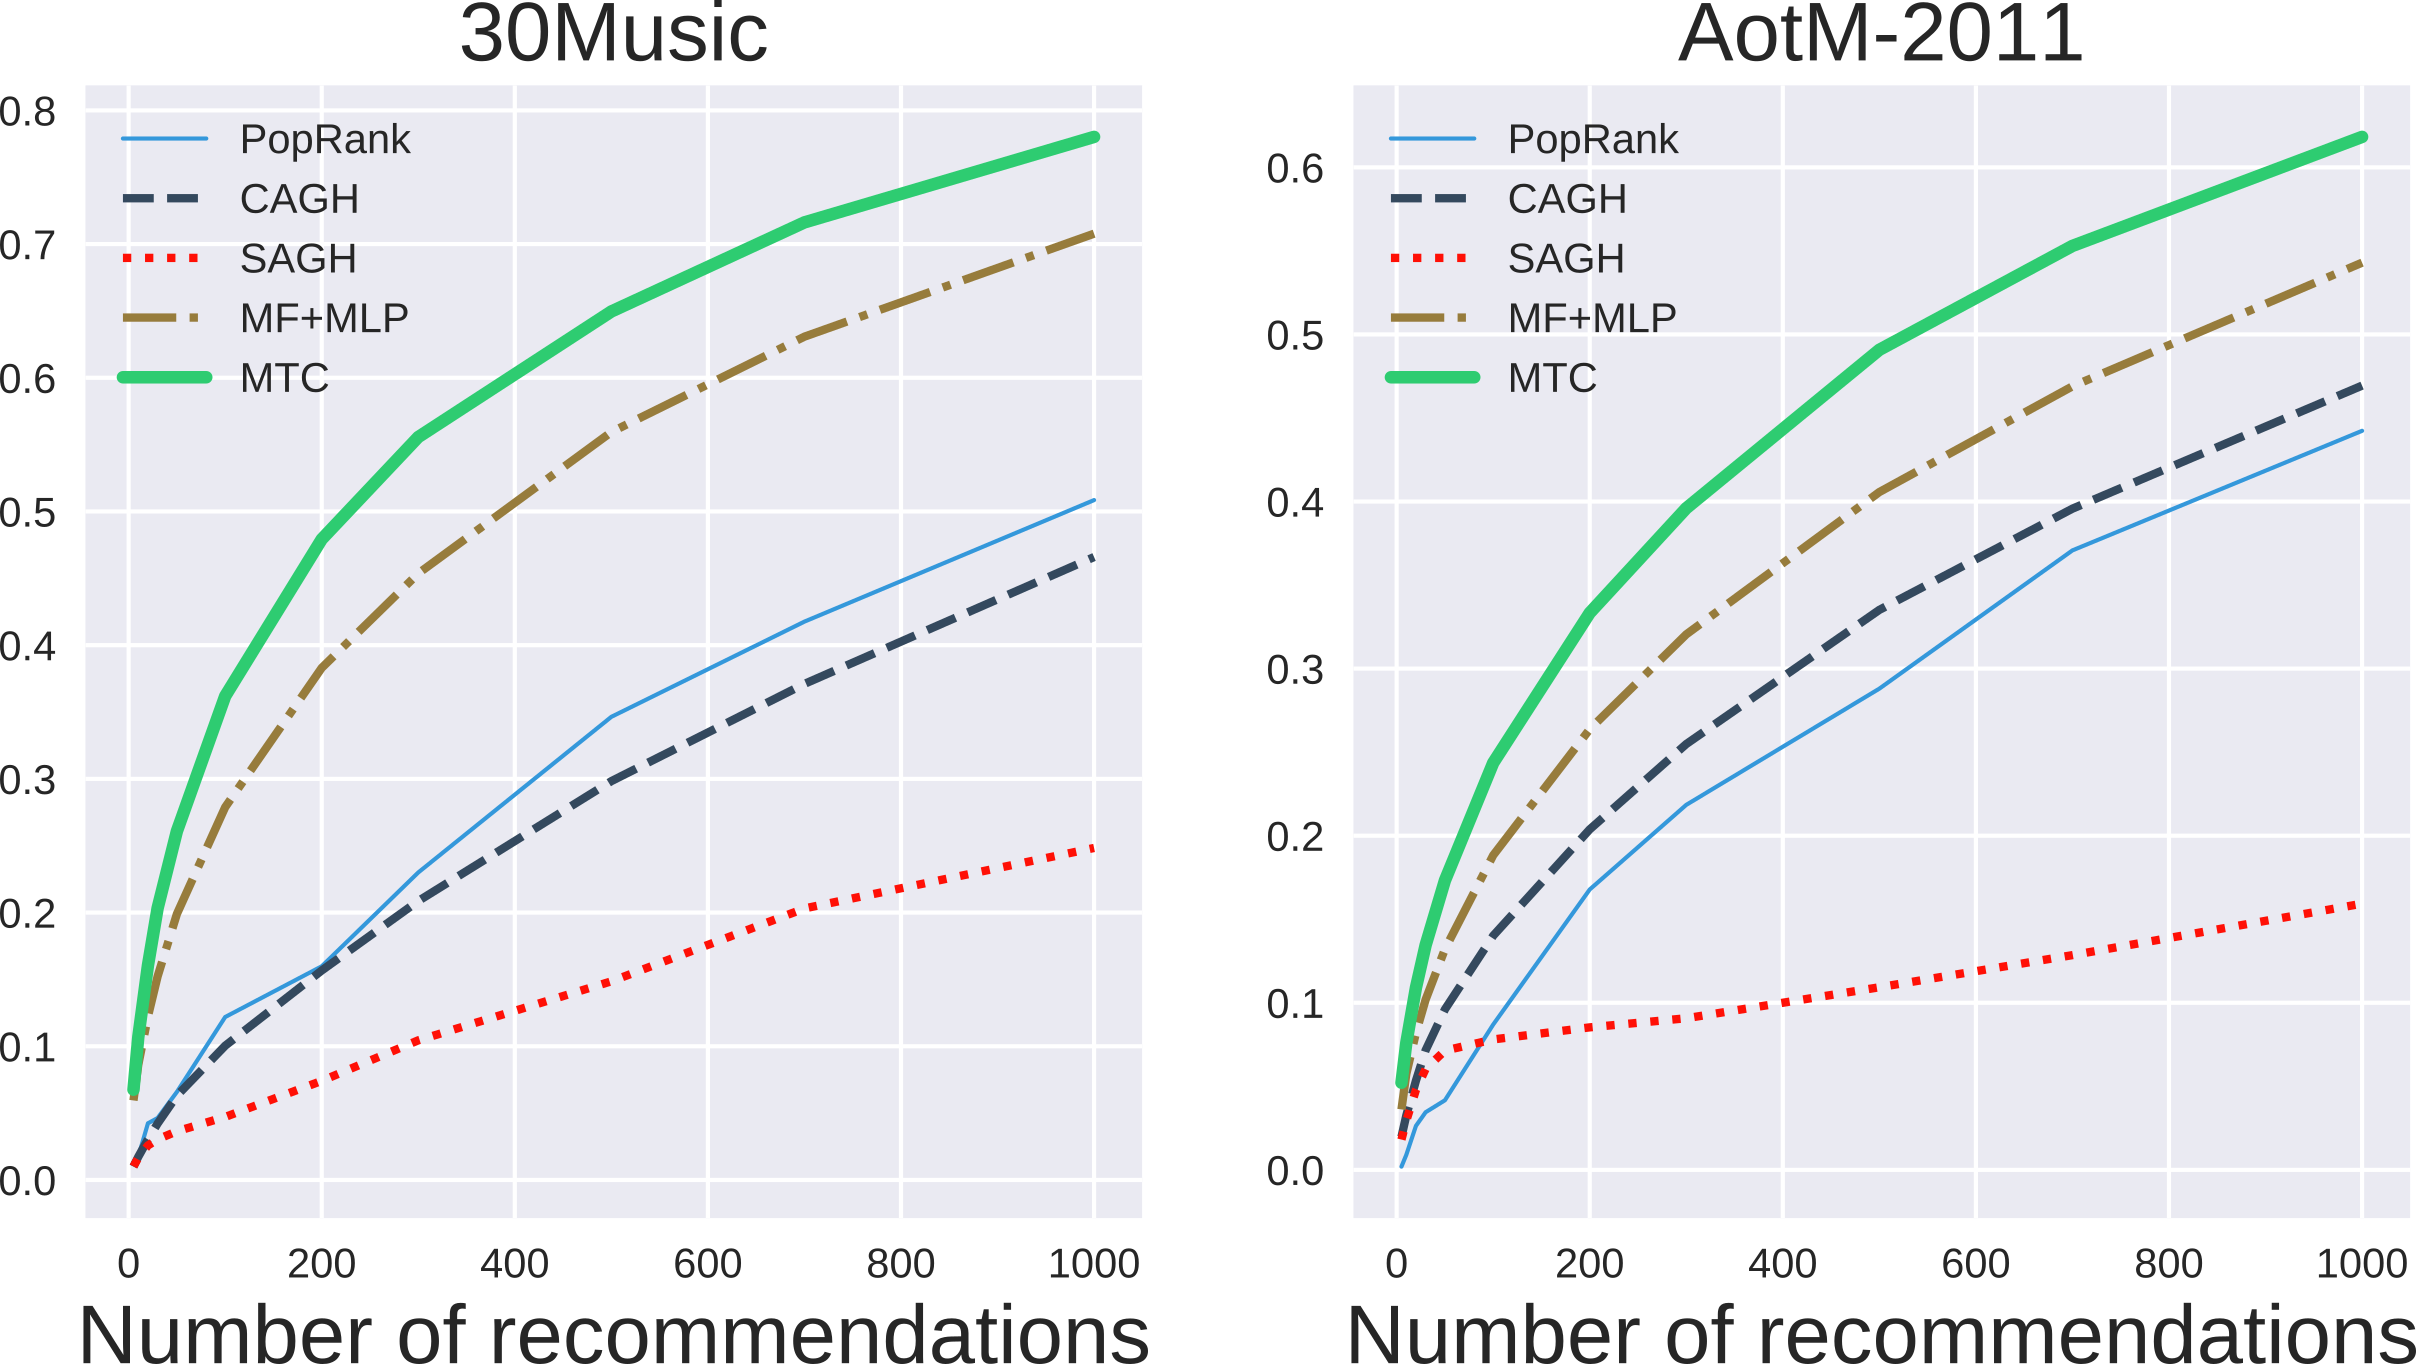
\includegraphics[width=\linewidth]{fig/hr1.png}
        \caption{Hit rates for {\it cold songs}}
        \label{fig:hr1}
    \end{minipage}
\end{figure*}

\begin{table}[t]
\caption{AUC for playlist recommendation in three cold-start settings, \emph{higher} values indicate better performance.}
\label{tab:auc}
\resizebox{\columnwidth}{!}{
%\resizebox{\textwidth}{!}{
\setlength\tabcolsep{2pt}
\begin{tabular}{lcccclcccclcccc}
\toprule 
\multicolumn{3}{c}{Cold Playlists} &&& \multicolumn{3}{c}{Cold Users} &&& \multicolumn{3}{c}{Cold Songs} \\ 
\cmidrule{1-3} \cmidrule{6-8} \cmidrule{11-13}
Method &  30Music &  AotM-2011 &&& 
Method &  30Music &  AotM-2011 &&& 
Method &  30Music &  AotM-2011 \\
\cmidrule{1-3} \cmidrule{6-8} \cmidrule{11-13}
%\midrule
PopRank & {\large 94.0}    & {\large 93.8}    \rule{0pt}{9pt} &&& 
PopRank & {\large 88.3}    & {\bf\large 91.8} \rule{0pt}{9pt} &&& 
PopRank & {\large 70.9}    & {\large 76.5}    \rule{0pt}{9pt} \\
%
CAGH    & {\large 94.8}    & {\large 94.2}    \rule{0pt}{9pt} &&& 
CAGH    & {\large 86.3}    & {\large 88.1}    \rule{0pt}{9pt} &&& 
CAGH    & {\large 68.0}    & {\large 77.4}    \rule{0pt}{9pt} \\
%                                            
SAGH    & {\large 64.5}    & {\large 79.8}    \rule{0pt}{9pt} &&&
SAGH    & {\large 54.5}    & {\large 53.7}    \rule{0pt}{9pt} &&&
SAGH    & {\large 51.5}    & {\large 53.6}    \rule{0pt}{9pt} \\
%                                          
WMF     & {\large 79.5}    & {\large 85.4}    \rule{0pt}{9pt} &&&
WMF+kNN & {\large 85.1}    & N/A              \rule{0pt}{9pt} &&&
MF+MLP  & {\large 81.4}    & {\large 80.8}    \rule{0pt}{9pt} \\
%
MTC     & {\bf\large 95.9} & {\bf\large 95.4} \rule{0pt}{9pt} &&&
MTC     & {\bf\large 89.6} & {\bf\large 91.8} \rule{0pt}{9pt} &&&
MTC     & {\bf\large 86.6} & {\bf\large 84.3} \rule{0pt}{9pt} \\
\bottomrule
\end{tabular}
}
\end{table}



\subsubsection{Baselines}
We compare the performance of our proposed method (\ie MTC) % (referred as {\it Multitask Classification}) 
with the following %a number of 
baseline approaches in each of the three cold-start settings:
%for the task of recommending music to form playlists:
\begin{itemize}
\item The {\it Popularity Ranking} (PopRank) method scores a song using only its popularity in the training set.
      In the \emph{cold songs} setting where song popularity is not available, 
      %we score a song using the popularity of the corresponding artist.
      a song is scored by the popularity of the corresponding artist.
\item The {\it Same Artists - Greatest Hits} (SAGH)~\cite{mcfee2012million} method scores a song
      by its popularity if the artist of the song appears in the given user's playlists (in the training set);
      otherwise the song is scored zero.
      In the {\it cold songs} setting, this method only considers songs from artists that appear in the given playlist,
      and scores a song using the popularity of the corresponding artist.
%      Similarly, we replace song popularity with artist popularity in the \emph{cold songs} setting.
\item The {\it Collocated Artists - Greatest Hits} (CAGH)~\cite{bonnin2013evaluating} method is a variant of SAGH.
      It scores a song using its popularity, but weighted by the frequency of the collocation between the artist of the song
      and artists that appear in the given user's playlists (in the training set).
      In the \emph{cold users} setting, we use the 10 most popular artists instead of artists 
      in the user's listening history, and the \emph{cold songs} setting is addressed in the same way as in SAGH.
%      The \emph{cold songs} setting is addressed in the same way as in SAGH.
%      as required by this method.
%\item The {\it Logistic Regression} baseline is specific for the \emph{cold songs} setting, where we independently learn 
%      a logistic regression classifier for each playlist, which is used to classify whether we should add each new song to 
%      this playlist\footnote{This method is also known as binary relevance in multi-label classification.}.
\item A variant of Matrix Factorisation (MF), which first learns the latent factors of songs, playlists
      or users through MF, then scores each song by the dot product of the corresponding latent factors.
      Recommendations are made as per the proposed method.
      In the \emph{cold playlists} setting, we factorise the song-user playcount matrix using the 
      weighted matrix factorisation (WMF) algorithm~\cite{hu2008collaborative}, which learns the 
      latent factors of songs and users.
      In the \emph{cold users} setting, we first learn the latent factors of songs and users using WMF,
      then approximate the latent factors of a new user by the average latent factors of the $k$ (\eg 100)
      nearest neighbours %\footnote{We choose $k=100$}
      (in terms of cosine similarity of user attributes, \eg age, gender and country) in the training set.
      We call this method WMF+kNN.
      \footnote{This method does not apply to the AotM-2011 dataset in the cold users setting,
      since such user attributes (\eg age, gender and country) are not available in the dataset.}
      In the \emph{cold songs} setting, we factorise the song-playlist matrix to learn the latent factors of 
      songs and playlists, which are then used to train a neural network to map song content features 
      to the corresponding latent factors~\cite{Gantner:2010,van2013deep}.
	  We can then obtain the latent factors of a new song as long as its content features are available.
      We call this method MF+MLP. 
%
%\item The three variants of Matrix Factorisation (MF), which first learn latent representations of songs, playlists or users
%      through MF, then score each song by the dot product of the song and the corresponding playlist or user latent factors.
%      Recommendations are made as per our method described in Section~\ref{sec:method}.
%      In the \emph{cold songs} setting, latent representations of songs/playlists are learnt by factorising the song-playlist matrix  
%      To obtain the representations of new songs, we learn a two-layer neural network (multilayer perceptron, MLP) to map song 
%      content features to the corresponding latent representations~\cite{Gantner:2010,van2013deep}, and call this method MF+MLP. 
%      In the \emph{cold playlists} setting, we factorise the song-user play-count matrix using the weighted matrix factorisation (WMF) 
%      algorithm~\cite{hu2008collaborative,van2013deep} to learn the latent representations of songs and users.
%      Similarly, latent representations of songs and users are learned using WMF in the \emph{cold users} setting, however, the latent 
%      factor of a new user is approximated by the mean factors of the $k$ nearest neighbours (in terms of cosine similarity of user 
%      attributes\footnote{User attributes include age, gender, country of the user, the number of playlists from her account, as well as 
%      her total play counts and subscription type, these attributes are only available in the 30Music dataset. We choose $k=100$.}) 
%      in training set, and we refer this method as WMF+kNN.
\end{itemize}


\subsubsection{Evaluation}

We evaluate %the performance of 
all approaches using two accuracy metrics that have been adopted 
in playlist recommendation tasks:
\emph{HitRate@K}~\cite{hariri2012context} and \emph{Area under the ROC curve} (AUC)~\cite{manning2008introIR}.
%In addition to these accuracy related metrics, 
We further adopt two beyond-accuracy metrics: %\ie
\emph{Novelty}~\cite{zhang2012auralist,schedl2017} and \emph{Spread}~\cite{kluver2014evaluating},
which are specifically tailored to recommender systems.
%Unlike the accuracy metrics, where higher values indicate better performance,
%\emph{moderate} values of Novelty and Spread are usually preferable~\cite{kluver2014evaluating,schedl2017}.
%
%R-Precision (RPREC) is the number of correctly recommended songs in the top-$n$ recommendation over $n$,
%where $n$ is the number of songs in the ground truth playlist.
%It is one of several metrics used to evaluate performance on playlist continuation tasks
%in the ACM RecSys Challenge 2018\footnote{https://recsys-challenge.spotify.com/rules}.

\emph{HitRate@K} (\ie Recall@K) 
is the number of correctly recommended songs amongst the top-$K$ recommendations over
%where $K$ is the number of recommendations, and $L$ is 
the number of songs in the %ground truth playlist. %\footnote{This metric is also known as Recall@K~\cite{schedl2017}.}.
observed playlist.
It has been widely employed to evaluate %several 
playlist generation and next song recommendation
methods~\cite{hariri2012context,bonnin2013evaluating,bonnin2015automated,jannach2015beyond}.
%
%The area under the ROC curve (AUC) 
AUC has been primarily used to measure the performance of classifiers.
It has been applied to evaluate %performance of 
playlist generation methods when the task
has been cast as a sequence of classification problems~\cite{ben2017groove}.

It is believed that
useful recommendations need to include previously unknown items~\cite{herlocker2004evaluating,zhang2012auralist}.
%and this 
This ability can be measured by \emph{Novelty},
which is based on the assumption that, intuitively, the more popular a song is, 
the more likely a user is to be familiar with it, and therefore the less likely to be novel.
%a user is more likely to be familiar with it, therefore less novel.
%
\emph{Spread}, however, is used to measure the ability of an algorithm to spread its attention across all possible songs.
It is defined as the entropy of the distribution of all songs.
See Appendix for more details of these beyond-accuracy metrics.


\subsection{Results and discussion}

\begin{figure}[!t]
    \centering
    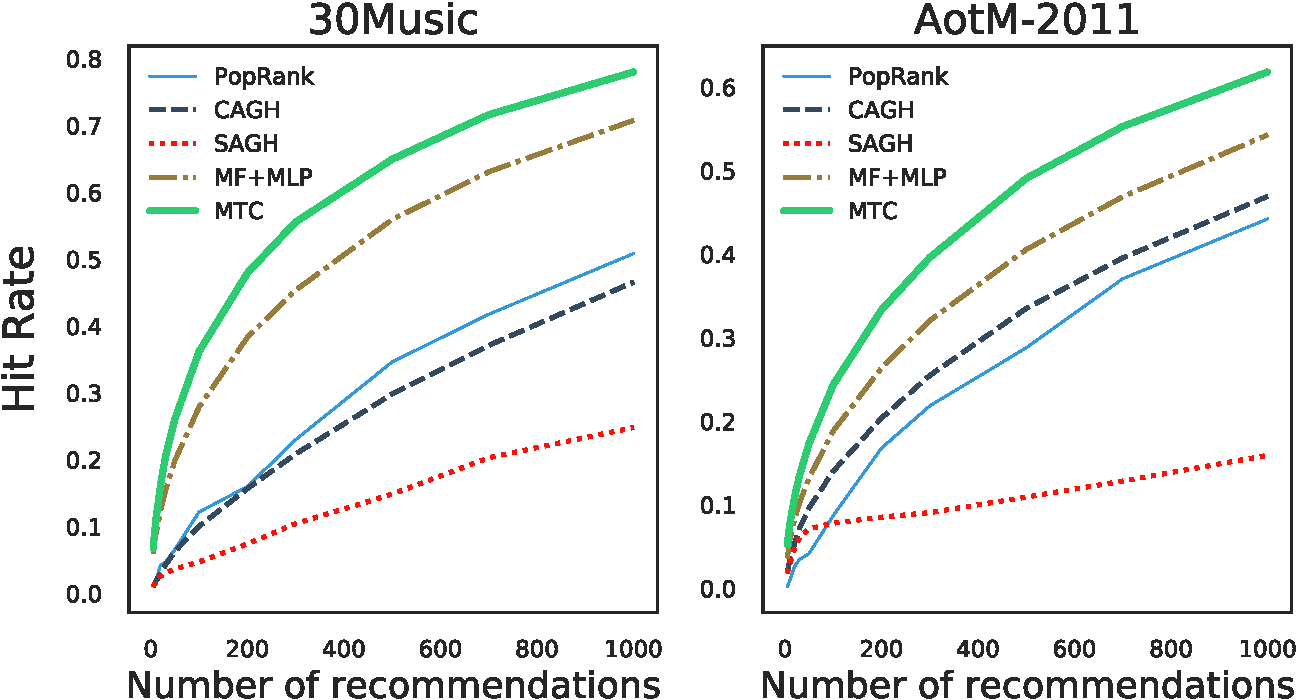
\includegraphics[width=\columnwidth]{fig/hr1.pdf}
    \caption{Hit rate of recommendation in the \emph{cold songs} setting.
\emph{Higher} values indicate better performance.}
    \label{fig:hr1}
\end{figure}

\begin{table}[!t]
\caption{Spread for playlist recommendation in three cold-start settings, \emph{moderate} values are preferable.}
\label{tab:spread}
\resizebox{\columnwidth}{!}{
\setlength\tabcolsep{2pt}
\begin{tabular}{lcccclcccclcccc}
\toprule 
\multicolumn{3}{c}{Cold Playlists} &&& \multicolumn{3}{c}{Cold Users} &&& \multicolumn{3}{c}{Cold Songs} \\ 
\cmidrule{1-3} \cmidrule{6-8} \cmidrule{11-13}
Method & 30Music & AotM-2011 &&& Method & 30Music & AotM-2011 &&& Method & 30Music & AotM-2011 \\ 
\cmidrule{1-3} \cmidrule{6-8} \cmidrule{11-13}
%\midrule
PopRank & {\large\: 9.8} & {\large  10.5} \rule{0pt}{9pt} &&&  
PopRank & {\large\: 9.8} & {\large  10.5} \rule{0pt}{9pt} &&&  
PopRank & {\large   7.4} & {\large   7.8} \rule{0pt}{9pt} \\
%                                      
CAGH    & {\large\: 5.8} & {\large\: 2.3} \rule{0pt}{9pt} &&&  
CAGH    & {\large\: 4.2} & {\large\: 5.3} \rule{0pt}{9pt} &&&  
CAGH    & {\large   4.3} & {\large   4.6} \rule{0pt}{9pt} \\
%                                      
SAGH    & {\large  10.3} & {\large  10.4} \rule{0pt}{9pt} &&&  
SAGH    & {\large  10.0} & {\large  10.7} \rule{0pt}{9pt} &&&  
SAGH    & {\large   6.5} & {\large   5.9} \rule{0pt}{9pt} \\
%
WMF     & {\large  10.7} & {\large  11.6} \rule{0pt}{9pt} &&&  
WMF+kNN & {\large  10.7} & N/A            \rule{0pt}{9pt} &&&
MF+MLP  & {\large   8.5} & {\large   9.2} \rule{0pt}{9pt} \\
%
MTC     & {\large\: 9.4} & {\large  10.4} \rule{0pt}{9pt} &&&  
MTC     & {\large\: 9.9} & {\large  11.4} \rule{0pt}{9pt} &&&  
MTC     & {\large   7.9} & {\large   8.3} \rule{0pt}{9pt} \\
\bottomrule
\end{tabular}
}
\end{table}


\subsubsection{Accuracy}

Table~\ref{tab:auc} shows the performance of all methods in terms of AUC.
We can see that PopRank %which simply ranking songs based on (song or artist) popularity 
achieves good performance in all three cold-start settings.
This is in line with results reported in~\cite{bonnin2013evaluating,bonnin2015automated}.
Artist information, particularly the frequency of artist collocations that is exploited in CAGH, 
improves recommendation in the cold playlists and cold songs settings.
Further, PopRank is one of the best performing methods in the cold users setting,
which is consistent with previous discoveries~\cite{mcfee2012million,bonnin2013evaluating,bonnin2015automated}.
The reason is believed to be the long-tailed distribution of songs in
playlists~\cite{cremonesi2010performance,bonnin2013evaluating}.
%
The MF variant does not perform well in the cold playlists setting,
but it performs reasonably well in the cold users setting when attributes of new users are available
(\eg in the 30Music dataset),
and it works particularly well in the cold songs setting where both song metadata and audio features are available 
for new songs.

Lastly, 
MTC is the (tied) best performing method in all three cold-start settings on both datasets.
Interestingly, it achieves the same performance as PopRank in the cold users setting on the AotM-2011 dataset,
which suggests that MTC might degenerate to simply ranking songs according to popularity when making recommendations
for new users; however, when attributes of new users are available, %(\eg in the 30Music dataset), 
it can improve 
%recommendations 
by exploiting information learned from existing users.


Figure~\ref{fig:hr1} shows the hit rate of all methods in the cold songs setting
%when the number of recommendations (\ie the number of recommended new songs) $K$ varies from 5 to 1000
when the number of recommended new songs varies from 5 to 1000.
As expected, the performance of all methods improves when the number of recommendations increases.
Further, we observe that learning based approaches (\ie MTC and MF+MLP) always perform better than 
% ranking based on artist information
other baselines that use only artist information.
%This demonstrates the effectiveness of learning from existing playlists for recommending new songs.
PopRank %that simply ranks new songs according to popularity of the corresponding artist
works surprisingly well;
it even outperforms CAGH which exploits artist collocations on the 30Music dataset.
The fact that CAGH always performs better than SAGH confirms that artist collocation is helpful
for music recommendation.
Lastly, MTC outperforms all other methods by a big margin on both datasets,
which demonstrates the effectiveness of the proposed approach for recommending new songs.

%We also observe that MTC %the multitask learning method proposed in this paper 
%improves over baseline approaches in the \emph{cold playlists} setting,
%and in the \emph{cold users} setting as well if a few user attributes are available,

We also observe that MTC improves over baselines in the cold playlists
and cold users settings (when simple attributes of new users are available),
although the margin is not as big as that in the cold songs setting.
See Appendix for details.
%although the improvement is not as big as that in the \emph{cold songs} settings.

%Interestingly, the CAGH method always performs better than SAGH, which may suggest that
%artist collocation is more informative that 

%Figure~\ref{fig:hr3} shows the hit rates of all methods in the \emph{cold playlists} setting
%when the number of recommendations $K$ varies from 5 to 1000.
%%It is not surprising that 
%As expected, the hit rates of all methods improves as the number of recommendations increases,
%We can also see that methods which use both song popularity and artist information outperform PopRank
%(except SAGH when $K$ is greater than 300).
%This is different from what we observed in Table~\ref{tab:auc},
%which suggest artist information is likely helpful to improve recall.
%Similar observations can be obtained in the cold users and cold songs setting, see Appendix for details. 


%\begin{table*}[!t]
%    \centering
%    \begin{tabular}{lr}
%    \begin{minipage}{.5\textwidth}
%        \begin{table}[t]
\caption{AUC for playlist recommendation in three cold-start settings, \emph{higher} values indicate better performance.}
\label{tab:auc}
\resizebox{\columnwidth}{!}{
%\resizebox{\textwidth}{!}{
\setlength\tabcolsep{2pt}
\begin{tabular}{lcccclcccclcccc}
\toprule 
\multicolumn{3}{c}{Cold Playlists} &&& \multicolumn{3}{c}{Cold Users} &&& \multicolumn{3}{c}{Cold Songs} \\ 
\cmidrule{1-3} \cmidrule{6-8} \cmidrule{11-13}
Method &  30Music &  AotM-2011 &&& 
Method &  30Music &  AotM-2011 &&& 
Method &  30Music &  AotM-2011 \\
\cmidrule{1-3} \cmidrule{6-8} \cmidrule{11-13}
%\midrule
PopRank & {\large 94.0}    & {\large 93.8}    \rule{0pt}{9pt} &&& 
PopRank & {\large 88.3}    & {\bf\large 91.8} \rule{0pt}{9pt} &&& 
PopRank & {\large 70.9}    & {\large 76.5}    \rule{0pt}{9pt} \\
%
CAGH    & {\large 94.8}    & {\large 94.2}    \rule{0pt}{9pt} &&& 
CAGH    & {\large 86.3}    & {\large 88.1}    \rule{0pt}{9pt} &&& 
CAGH    & {\large 68.0}    & {\large 77.4}    \rule{0pt}{9pt} \\
%                                            
SAGH    & {\large 64.5}    & {\large 79.8}    \rule{0pt}{9pt} &&&
SAGH    & {\large 54.5}    & {\large 53.7}    \rule{0pt}{9pt} &&&
SAGH    & {\large 51.5}    & {\large 53.6}    \rule{0pt}{9pt} \\
%                                          
WMF     & {\large 79.5}    & {\large 85.4}    \rule{0pt}{9pt} &&&
WMF+kNN & {\large 85.1}    & N/A              \rule{0pt}{9pt} &&&
MF+MLP  & {\large 81.4}    & {\large 80.8}    \rule{0pt}{9pt} \\
%
MTC     & {\bf\large 95.9} & {\bf\large 95.4} \rule{0pt}{9pt} &&&
MTC     & {\bf\large 89.6} & {\bf\large 91.8} \rule{0pt}{9pt} &&&
MTC     & {\bf\large 86.6} & {\bf\large 84.3} \rule{0pt}{9pt} \\
\bottomrule
\end{tabular}
}
\end{table}

%    \end{minipage}%
%    &
%    \begin{minipage}{.5\textwidth}
%        \begin{table}[!t]
\caption{Spread for playlist recommendation in three cold-start settings, \emph{moderate} values are preferable.}
\label{tab:spread}
\resizebox{\columnwidth}{!}{
\setlength\tabcolsep{2pt}
\begin{tabular}{lcccclcccclcccc}
\toprule 
\multicolumn{3}{c}{Cold Playlists} &&& \multicolumn{3}{c}{Cold Users} &&& \multicolumn{3}{c}{Cold Songs} \\ 
\cmidrule{1-3} \cmidrule{6-8} \cmidrule{11-13}
Method & 30Music & AotM-2011 &&& Method & 30Music & AotM-2011 &&& Method & 30Music & AotM-2011 \\ 
\cmidrule{1-3} \cmidrule{6-8} \cmidrule{11-13}
%\midrule
PopRank & {\large\: 9.8} & {\large  10.5} \rule{0pt}{9pt} &&&  
PopRank & {\large\: 9.8} & {\large  10.5} \rule{0pt}{9pt} &&&  
PopRank & {\large   7.4} & {\large   7.8} \rule{0pt}{9pt} \\
%                                      
CAGH    & {\large\: 5.8} & {\large\: 2.3} \rule{0pt}{9pt} &&&  
CAGH    & {\large\: 4.2} & {\large\: 5.3} \rule{0pt}{9pt} &&&  
CAGH    & {\large   4.3} & {\large   4.6} \rule{0pt}{9pt} \\
%                                      
SAGH    & {\large  10.3} & {\large  10.4} \rule{0pt}{9pt} &&&  
SAGH    & {\large  10.0} & {\large  10.7} \rule{0pt}{9pt} &&&  
SAGH    & {\large   6.5} & {\large   5.9} \rule{0pt}{9pt} \\
%
WMF     & {\large  10.7} & {\large  11.6} \rule{0pt}{9pt} &&&  
WMF+kNN & {\large  10.7} & N/A            \rule{0pt}{9pt} &&&
MF+MLP  & {\large   8.5} & {\large   9.2} \rule{0pt}{9pt} \\
%
MTC     & {\large\: 9.4} & {\large  10.4} \rule{0pt}{9pt} &&&  
MTC     & {\large\: 9.9} & {\large  11.4} \rule{0pt}{9pt} &&&  
MTC     & {\large   7.9} & {\large   8.3} \rule{0pt}{9pt} \\
\bottomrule
\end{tabular}
}
\end{table}

%    \end{minipage}%
%    \end{tabular}
%\end{table*}


%\subsubsection{Novelty and spread}
\subsubsection{Beyond accuracy}

%Unlike the accuracy metrics, 
Note that, unlike AUC and hit rate,
where higher values indicate better performance,
\emph{moderate} values of Spread and Novelty are usually preferable~\cite{kluver2014evaluating,schedl2017}.

Table~\ref{tab:spread} shows the performance of all recommendation approaches in terms of \emph{Spread}.
In the cold songs setting, CAGH and SAGH focus on songs from artists in users' listening history and similar artists, 
which explains the relative low \emph{Spread}.
However, in the cold playlists and cold users settings, 
SAGH improves its attention spreading due to the set of songs it focuses on is significantly bigger 
(\ie songs from all artists in users' previous playlists and songs from the 10 most popular artists, respectively).
Surprisingly, CAGH remains focusing on a relatively small set of songs in both settings.
Lastly, in all three cold-start settings, the MF variants have the highest \emph{Spread},
while both PopRank and MTC have (similar) moderate \emph{Spread},
which is considered better. %to have better performance.


%We can see from Table~\ref{tab:spread} that both PopRank and MTC can similarly spread the attention across 
%all possible songs in all three cold-start settings. 
%In the cold songs setting, CAGH and SAGH focus on songs from artists in users' listening history and similar artists, 
%which explains the relative low spread values.
%However, in the cold playlists and cold users settings, SAGH improves its attention spreading due to the set of songs 
%it focuses on is significantly bigger (\ie songs from all artists in users' previous playlists and the top-10 
%most popular artists, respectively).
%Surprisingly, CAGH remains focuses on a relatively small set of songs in both settings.
%Lastly, the Matrix Factorisation variants can generally spread the attention cross 
%all possible songs comparably well.


Figure~\ref{fig:nov3} shows the \emph{Novelty} of all methods in the cold playlists setting.
We can see that PopRank has the lowest \emph{Novelty},
which is not surprising given the definition of \emph{Novelty} (see Appendix).
Both SAGH and CAGH start with low \emph{Novelty} and grow when the number of recommended songs increases,
%Interestingly, SAGH grows much faster compared  CAGH
but the \emph{Novelty} of CAGH saturates much earlier than that of SAGH.
The reason could be that,
when the number of recommendations is larger than the total number of songs from artists in a user's previous playlists,
SAGH will simply recommend songs randomly (which are likely to be novel)
while CAGH will recommend songs from artists that are similar to those in a user's previous playlists
%(which are probably less novel).
(which could be comparably less novel).
Further, MTC achieves lower \emph{Novelty} than WMF and CAGH, 
which indicates that MTC tends to recommend popular songs to form new playlists. %for existing users.
To conclude, 
MTC and CAGH have moderate \emph{Novelty} on both datasets,
and therefore perform better than other approaches.

The proposed approach also achieves moderate \emph{Novelty} in the cold songs setting.
%but performs similar to PopRank in the cold users setting.
However, in the cold users setting, the MF variant and CAGH have moderate \emph{Novelty},
which are therefore preferred. See Appendix for details.


%From Figure~\ref{fig:nov1} we can see that PopRank achieves the lowest Novelty,
%which is not surprising given the definition of Novelty.
%The Novelty of SAGH increases dramatically when the number of recommendations is larger than 30 or 50, 
%the reason could be the average numbers of songs from an artist is around between 30 and 50 
%as shown in Table~\ref{tab:stats_pldata}, and SAGH simply recommends random
%songs from artists that do not appear in users' listening history.
%All other methods achieve moderate Novelty and hence perform better for recommending new songs.
%
%Similar observations can be obtained from Figure~\ref{fig:nov3} for the cold playlists recommendation.
%However, there are two differences: 
%(i) the Novelty of SAGH increases less dramatically due to the set of songs being considered are from
%all artists of users' previous playlists; 
%(ii) the proposed method MTC achieves lower Novelty (in general) than CAGH and WMF, 
%which indicates that MTC trends to prefer popular songs to form new playlists for existing users.

%It is interesting to see that, the MTC and PopRank perform identically in the cold users setting~(Figure~\ref{fig:nov4}),
%which provides more evidence that MTC degenerates to rank songs according to popularity.
%CAGH and the variant of Matrix Factorisation generally perform better 
%(in terms of Novelty) for recommending playlists for new users.


\begin{figure}[!t]
    \centering
    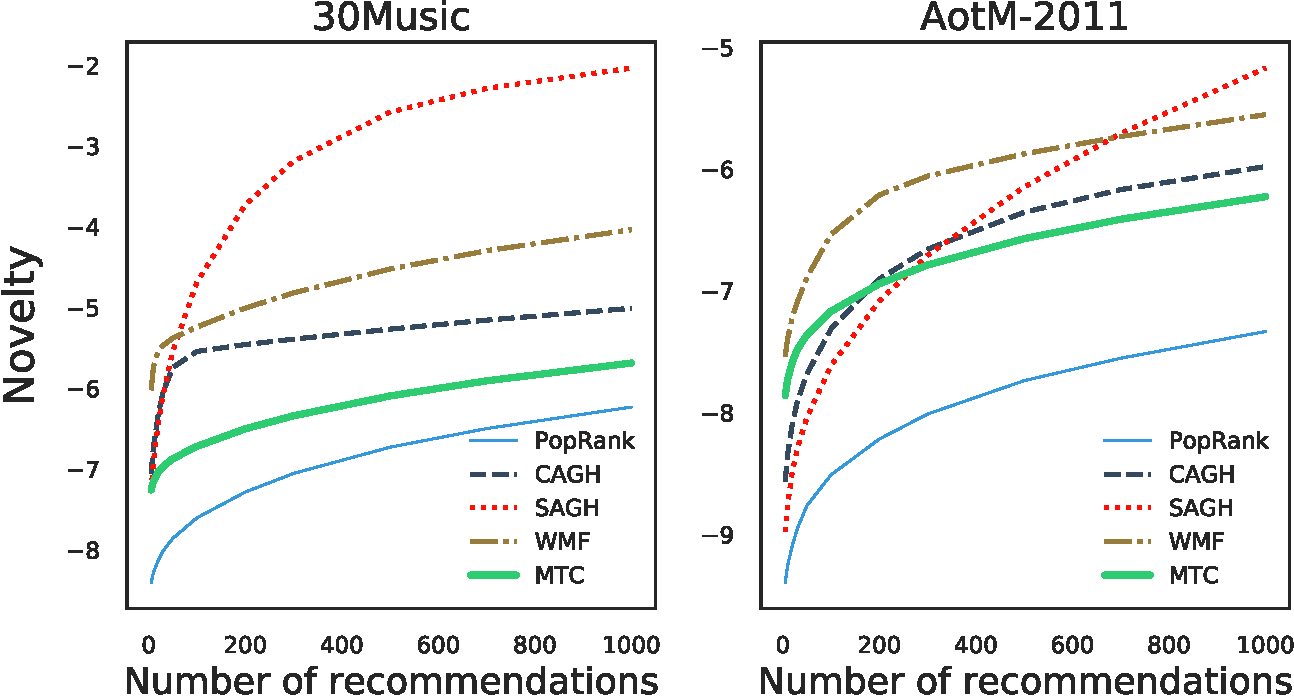
\includegraphics[width=\columnwidth]{fig/nov3.pdf}
    \caption{Novelty of recommendation in the \emph{cold playlists} setting.
\emph{Moderate} values are preferable.}
    \label{fig:nov3}
\end{figure}


%\begin{figure}[!t]
%    \centering
%    \begin{subfigure}[t]{\columnwidth}
%        \centering
%        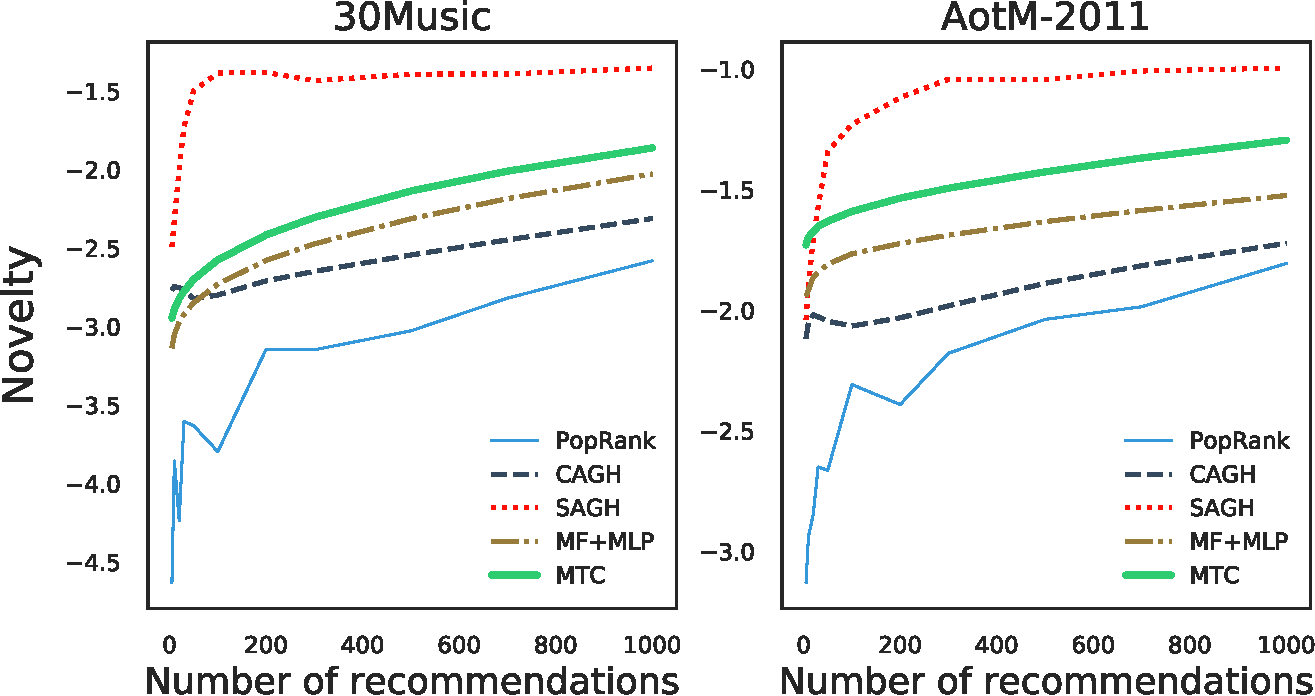
\includegraphics[width=\columnwidth]{fig/nov1.pdf}
%        \caption{Cold Songs}
%        \label{fig:nov1}
%    \end{subfigure}
%    \begin{subfigure}[t]{\columnwidth}
%        \centering
%        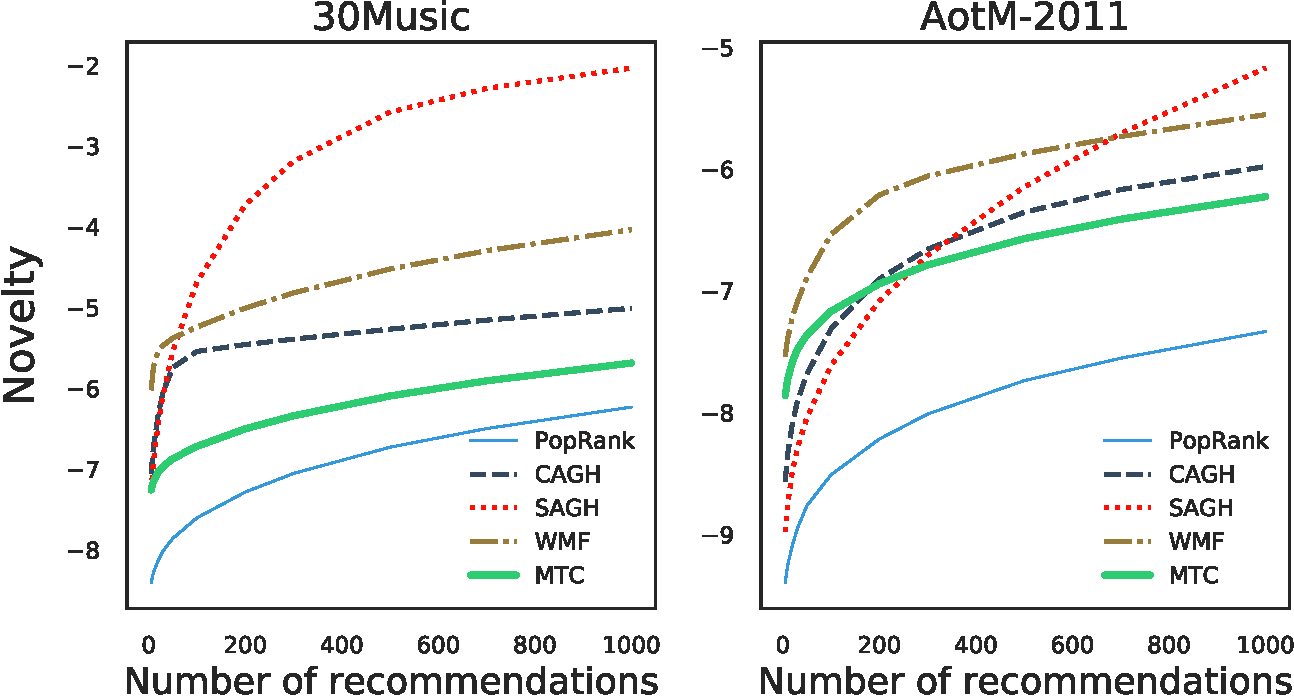
\includegraphics[width=\columnwidth]{fig/nov3.pdf}
%        \caption{Cold Playlists}
%        \label{fig:nov3}
%    \end{subfigure}
%    \caption{Novelty of cold-start recommendations, \emph{moderate} values are preferable.}
%\end{figure}
